\section{ECS als relationales Modell}

Im folgenden Abschnitt motivieren wir die idiomatische ECS-Datenstruktur auf Grundlage des relationalen Modells.\\
Mit Hilfe von funktionalen Abhängigkeiten weisen wir die Normalenformen nach, um im Weiteren mit Normalformtheorien zusammenhängende Lösch- und Aktualisierungsanomalien formal ausschließen zu können.\\
Ausgehend von einem breiten Relationsschema überführen wir den Entwurf in ein ECS-idiomatisches komponentenzentrisches Modell und weisen hierfür die 6te Normalform nach.

\subsubsection*{Hinweise zur Notation}
Bei Begriffen und Notation folgen wir der üblichen Fachliteratur, insbesondere Elmasri und Navathe~\cite{EN11}.\\
Mit Blick auf die Relationen zwischen Entität und Komponenten bezeichnen wir das relationale Modell des ECS im Folgenden als \textit{ECS-Modell}.
Wo sich die Erweiterungen des Modells nicht aus dem Kontext ergeben, wird entsprechend erklärend darauf hingewiesen.\\
Um der übrigen Notation in dieser Arbeit gerecht zu bleiben, verwenden wir auch in diesem Abschnitt für die Subskripte der Komponententypen Buchstaben.
Wo der Zusammenhang erfordert, ersetzen wir die Buchstaben durch Ziffern, um beispielsweise deutlicher auf eine endliche Menge von Komponentenassoziationen hinzuweisen; diese setzen wir aber stets -- unabhängig von der Schreibweise -- implizit voraus.
Der binäre Natural-Join-Operator $\njoin$ wird im Kontext von Relationszuständen $\pi_{R_n}(r)$ in der Form
\[
    \njoin (\pi_{R_1}(r), \ldots, \pi_{R_n}(r)),\ n \in \mathbb{N}
\]
\noindent
genutzt, um den durch die Join Operation
\[
     \pi_{R_1}(r) \njoin \ldots \njoin \pi_{R_n}(r))
\]
\noindent
ergebenden Relationszustand $r$ zu notieren.\\

\noindent
Im Folgenden schließt \textit{verlustfrei} im Zusammenhang mit Joins und Zerlegung auch immer die Eigenschaft \textit{nicht-additiv} mit ein.\\
Funktionale Abhängigkeit(en) wird im Folgendem mit FD(s) abgekürzt.\\
Mehrwertige Abhängigkeiten werden mit MVD abgekürzt.

\subsection{Das relationale Schema}
Ein erster Entwurf eines relationalen Schemas, dass die Beziehungen zwischen \textit{Entität} und \textit{Komponenten} ausdrückt, führt zu dem in Abbildung~\ref{fig:relation} dargestellten Modell.
Der Entitätstyp $E$ ist dort mit zwei Komponententypen $K_i$, $K_j$ dargestellt, wobei die Beziehungen als  binäre Relationen modelliert sind -- die Darstellung entspricht damit dem \textit{entitätszentrischen} Ansatz und wird schematisch in ähnlicher Form bei Redmond et {al.} verwendet~\cite[Fig.1, 272:3]{RCCM+25}.


\begin{figure}[!htbp]
    \centering
    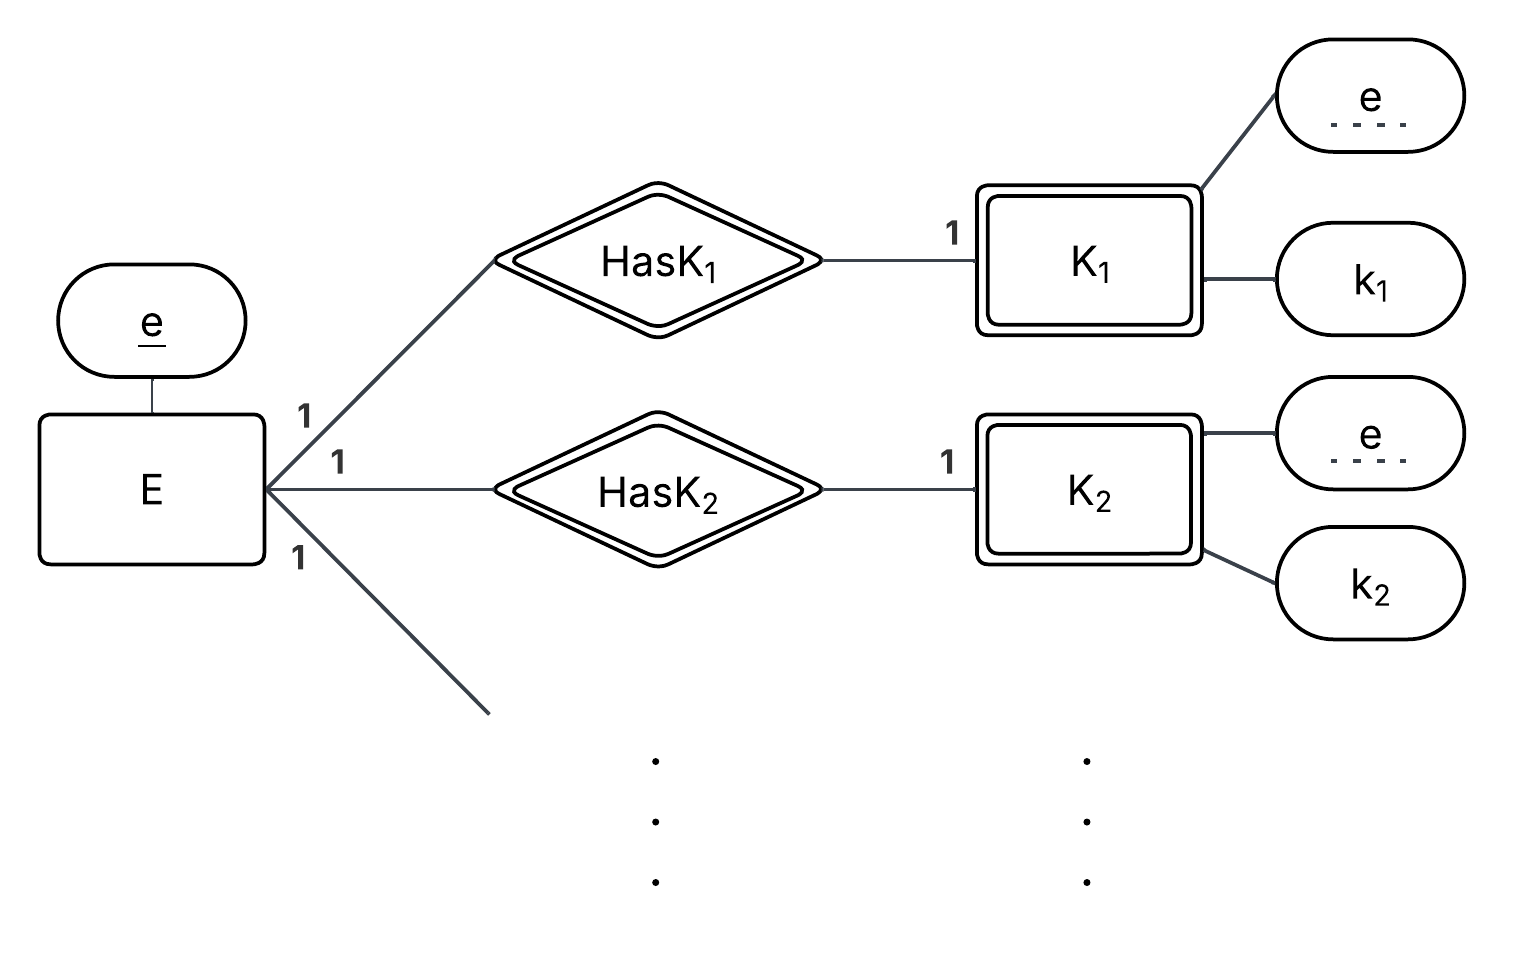
\includegraphics[width=0.6\columnwidth]{content/de/appendix/concurrency_paper/notation/img/relation}
    \caption{Entitätszentrischer Entwurf eines Entity-Relationship-Modells von Entität und Komponenten.
    Relationen sind identifizierend modelliert, da ein Komponententerm $k_i$ nicht ohne eine besitzende Entität existieren kann.
    Entsprechend sind $K_i, K_j, \ldots$ als schwache Typen modelliert, die über $E$ identifiziert werden. Die Notation folgt der Chen-Notation~\cite{Che76}. (Quelle: eigene Darstellung)}
    \label{fig:relation}
\end{figure}

\subsection{Funktionale Abhängigkeiten im ECS-Modell}

Relation und Attributmengen des ECS-Modells ergeben sich wie folgt:

\[
    \begin{alignat}{3}
        &E   &&= \{e\}\\
        &K_i &&= \{e, k_i\}\\
        &K_j &&= \{e, k_j\}\\
        &K_k &&= \{e, k_k\}\\
        & \ldots
    \end{alignat}
\]

\noindent
Als Primärschlüssel für $E$ identifizieren wir das Attribut $e$.
In den Relationen $K_i, K_j, \ldots$ ist $e$ der Fremdschlüssel; zusammen mit der 1:1 Kardinalität der Relationen auch gleichzeitig der Primärschlüssel.\\

\noindent
Die funktionalen Abhängigkeiten der Relationen lauten:

\[
    \begin{alignat}{3}
        F_E = &\{ e \rightarrow e\}\\
        F_{K_i} = &\{ e \rightarrow k_i\}\\
        F_{K_j} = &\{ e \rightarrow k_j\}\\
        \ldots
    \end{alignat}\
\]
\medskip

\noindent
Mit diesen Informationen können wir das Universalrelationsschema

\[
 K(e, k_i, k_j, k_k, \ldots)
\]
\smallskip

\noindent
ableiten, das in Abbildung~\ref{fig:universalrelation_k} dargestellt ist.\\

\begin{figure}[!htbp]
    \centering
    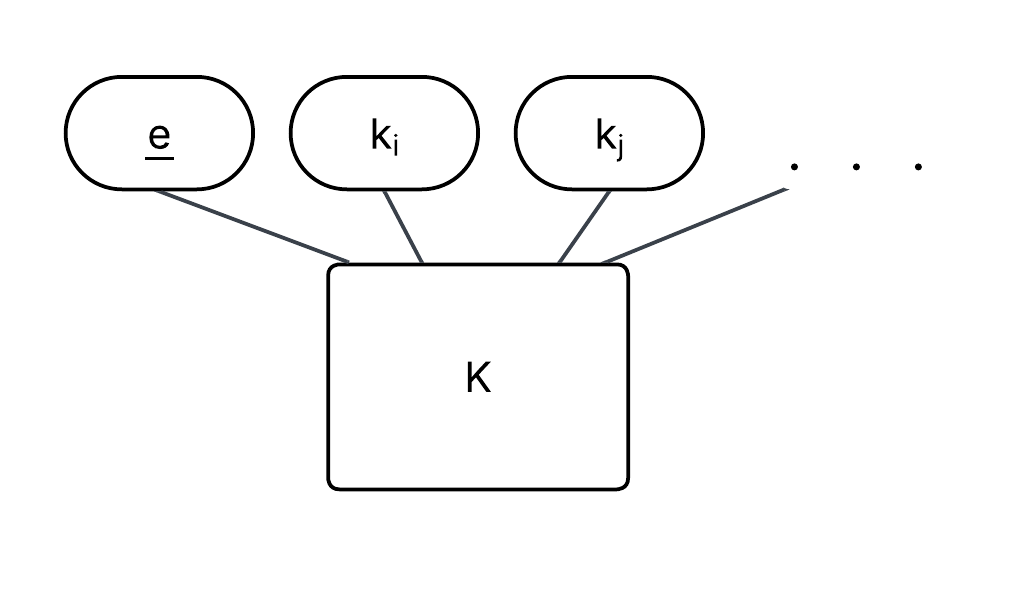
\includegraphics[width=0.6\columnwidth]{content/de/appendix/concurrency_paper/notation/img/universalrelation_k}
    \caption{Komponenten und Entität zusammengeführt in der Relation $K$. (Quelle: eigene Darstellung)}
    \label{fig:universalrelation_k}
\end{figure}

\noindent
Die funktionalen Abhängigkeiten $F_K$ von $K$ ergeben sich damit zu

\[
    \begin{alignat}{3}
         F_K &= F_E \cup F_{K_i} \cup F_{K_j} \cup \ldots =
            &\{e \rightarrow e, e \rightarrow k_i, \ e \rightarrow k_j, \ \ldots\}
    \end{alignat}
\]
\medskip

\noindent
Die Hülle von $e$ unter $F_K$ lautet:

\[
    e^+ =\{e, k_i, k_j, k_k, \ldots\}
\]

\noindent
Folglich ergibt sich die minimale funktionale Abhängigkeitsmenge $F^\text{min}_{K}$ zu:
\[
    \begin{alignat}{3}
        F^\text{min}_{K} = &\{e \rightarrow {k_i},\ e \rightarrow {k_j}, \ e \rightarrow {k_k}, \ \ldots  \}
    \end{alignat}
\]

\noindent
Daraus folgt
\[
    \begin{alignat}{3}
        (F^\text{min}_{K})^+ = (F_{K})^+
    \end{alignat}
\]


\subsection*{Darstellung fehlender Komponenten im Universalrelationsschema}

In dem breiten Relationsschema $K$ ist es nicht möglich, ohne speziellen Wert die Abwesenheit einer Komponente für eine Entität darzustellen: So kann im Relationszustand $r$ ein Tupel
\[
    t \in \pi_{K}(r)
\]
\noindent
nur existieren, wenn folgendes erfüllt ist:

\[
    \forall v_i \in \{t[A_i] \mid t \in \pi_{K}(r)\}: v_i \in dom(A_i)
\]

\noindent
mit
\[
    A_i \in K\backslash \{e\}, i \in I
\]

\noindent
Damit kann eine Entität, die eine Assoziation zu $K_\text{Position}$ hat, aber keine Assoziation zu $K_\text{Velocity}$, nicht Teil des Relationszustands $\pi_{K}(r)$ sein.\\

\noindent
Anstatt einen \text{NULL}-Wert für diese Fälle einzuführen, übernehmen wir in Anlehnung an Redmond et {al.} den Unit-Wert $\unitval$ vom Typ $\top$.\footnote{
    Damit können wir eine Brücke hin zu der Typ- als auch der Funktionssemantik des bei Redmond et {al.} verwendeten konjunktiven Anfragesystems bauen, ohne weitere Konventionen oder Voraussetzungen, die mit \text{NULL}-Werten einhergehen könnten, für das relationale Modell zu erzwingen.
}
Damit erweitern wir die Wertebereiche auf $K_i + \top,\ K_j + \top, \ldots$, so dass für die Attribute auf eine erweiterte Wertemenge zurückgegriffen werden kann:

\[
\begin{alignedat}{3}
  \text{dom}(k_i) &= K_i + \top\\
  \text{dom}(k_j) &= K_j + \top\\
    \ldots
\end{alignedat}
\]

\noindent
Die um $\top$ erweiterten Komponententypen, Relationen und Attribute notieren wir im Folgenden mit einem Superscript $^\top$:\\

\[
    K^{\top}(e, \ k_i^\top, k_j^\top, \ldots)
\]

\noindent
Die im vorherigen Abschnitt angegebenen funktionalen Abhängigkeiten und Abhängigkeitsmengen ändern sich damit nicht, abgesehen der geringfügig abweichenden Notation, beispielsweise für $F^\text{min}_{K^\top}$:

\[
    F^\text{min}_{K^\top} = \{e \rightarrow k^\top_1, e \rightarrow k^\top_2, \ldots e \rightarrow k^\top_n \}
\]

\bigskip
\begin{tcolorbox}[title={Zusätzliche Integritätsbedingung für $K^{\top}$}]
Als zusätzliche Integritätsbedingung kann vereinbart werden, dass eine Entität nicht ausschließlich $\unitval$-Werte in den Komponentenattributen aufweisen darf.
Ein Tupel der Relation $K^\top$ im Relationszustand $\pi_{K^\top}(r)$ muss mindestens einen konkreten Komponententerm aufweisen.
\[
    \forall t \in \pi_{K^\top}(r), A_i \neq e: \exists t[A_i]: t[A_i] \neq \unitval
\]
\end{tcolorbox}

\subsection*{Nachweis der Normalformen}

Wir führen im folgenden den Nachweis der 1., 2., 3., 4., und 5. sowie der Boyce-Codd-Normalform.
Wie beginnen zunächst mit einigen Hilfssätzen, die den Nachweis erleichtern.\\


\bigskip
\begin{axiom}\label{ax:nur_atomar}
    Die Wertemengen der Attribute von $K^\top$ lassen nur einzelne, untrennbare (und damit atomare) Werte zu.
\end{axiom}

\bigskip
\begin{axiom}\label{ax:einfacher_schluessel}
    Der einzige Schlüsselkandidat der Relation $K^\top$ ist $e$.
\end{axiom}
\bigskip

\begin{definition}\label{def:entitätsbezogen}

    Eine Relation $K^\top_i$, für die $e \in K^\top_i$ gilt, ist eine \textit{entitätsbezogene Relation}.\\

    \noindent
    Eine Zerlegung $D = (K^\top_1, K^\top_2, \ldots, K^\top_m)$ von $K^\top$ mit

    \[
        K^\top_1 \cup K^\top_2 \cup \ldots \cup K^\top_m = K^{\top}
    \]
die ausschließlich entitätsbezogene Relationen enthält, bezeichnen wir als \textit{entitätsbezogene Zerlegung}.
\end{definition}


\bigskip
\begin{lemma}\label{lem:K_bin_ist_verlustfrei}
    Die entitätsbezogene Relation $K_{ij}^\top = K(e, k^\top_i, k^\top_j)$ lässt sich verlustfrei in entitätsbezogene Relationen $K^\top_i(e, k^\top_i), K^\top_j(e, k^\top_j)$ zerlegen.
\end{lemma}

\medskip
\begin{proof}
    Sei $K^{\top}_i = \pi_{(e, k^{\top}_i)}(K_{ij}^\top),\ K^{\top}_j = \pi_{e, k^{\top}_j}(K_{ij}^\top)$.\\

    \noindent
    Wir zeigen, dass
    \[
        \pi_{K^{\top}_i}(r)\ \bowtie_{K^{\top}_i.e = K^{\top}_j.e}\ \pi_{K^{\top}_j}(r) = \njoin\ (\pi_{K^{\top}_i}(r), \pi_{K^{\top}_j}(r)) = \pi_{K_ij^\top}(r)
    \]

    \bigskip
    \noindent
    Da es sich um eine binäre Zerlegung handelt, kann der Beweis anhand der funktionalen Eigenschaften erfolgen~\cite[S. 343]{EN11}:
    \[
        \begin{alignedat}{3}
            ((K^{\top}_i \cap K^{\top}_j) &\rightarrow (K^{\top}_i - K^{\top}_j)) = (e \rightarrow k^{\top}_i\ ) \in e^{+\top}\\
            (K^{\top}_i \cap K^{\top}_j) &\rightarrow (K^{\top}_j - K^{\top}_i)) = (e \rightarrow k^{\top}_j) \in e^{+\top}\\
        \end{alignedat}
    \]
\end{proof}



\bigskip
\begin{lemma}\label{lem:K_plus_ist_verlustfrei}
    Die Relation $K^\top = K(e, k^\top_1, k^\top_2, \ldots, k^\top_n), n \geq 2$ lässt sich verlustfrei entitätsbezogen nach $D= (K^\top_1, K^\top_2, \ldots, K^\top_m, m \geq 2)$ zerlegen.
\end{lemma}

\medskip
\begin{proof}
    Um Lemma~\ref{lem:K_bin_ist_verlustfrei} auf m-äre Zerlegungen $\pi_{K^{\top}_1}(r), \pi_{K^{\top}_2}(r), \ldots, \pi_{K^{\top}_m}$ von $K^\top$ auszuweiten, ist zu zeigen:
    \[
        \pi_{{K^\top}}(r) =\ \njoin (\pi_{K^{\top}_1}(r), \pi_{K^{\top}_2}(r), \ldots, \pi_{K^{\top}_m}(r))
    \]

    Hierzu wenden wir das Chase-Verfahren an~\cite{ABU79}~\cite[Algorithmus 10.2, S. 342]{EN11}.
    Für eine bessere Lesbarkeit verzichten wir in der Tableaudarstellung auf die $b$-Symbole und nutzen stattdessen Unterstriche $\_$ in entsprechenden Zellen.\\

    \noindent
    Die Zerlegung der einzelnen Relationen erfolgt zunächst entitätsbezogen nach Definition~\ref{def:entitätsbezogen} , so dass
    \[
        \forall K^{\top}_i \in D : e \in K^{\top}_i,\quad \lvert K^{\top}_i \rvert \geq 2
    \]
    Damit ist sichergestellt, dass der Primärschlüssel von $K^\top$ Attribut jeder Relation ist.

    \noindent
    Sei zunächst wie in dem Verfahren angegeben das Tableau wie folgt aufgebaut:
    Spalten entsprechend den Attributnamen von $K^\top$, in der Reihenfolge $e, k_1^{\top}, \ldots, k_n^\top$.
    Die Zeilen sind mit den Relationsnamen $K^\top_1, K^\top_2, \ldots, K^\top_m$ der Zerlegung markiert.
    Wir erhalten dadurch folgendes Tableau, wobei $\circ$ als Platzhalter für die jeweiligen Zelleninhalte steht:\\

    \[
        \begin{array}{c|cccccc}
            & e      & k^{\top}_1 & k^{\top}_2 & k^{\top}_3 & \dots  & k^{\top}_n \\
            \hline
            K^{\top}_1      & \circ     & \circ         & \circ         & \circ         & \dots  & \circ         \\
            K^{\top}_2      & \circ     & \circ         & \circ         & \circ         & \dots  & \circ         \\
            K^{\top}_3      & \circ     & \circ         & \circ         & \circ         & \dots  & \circ         \\
            \vdots          & \vdots & \vdots     & \vdots     & \vdots     & \ddots & \vdots     \\
            K^{\top}_m      & \circ     & \circ         & \circ         & \circ         & \dots  & \circ
        \end{array}
    \]
\medskip

    Entsprechend der Vorschrift des Verfahrens gilt in unserem Fall, dass für jede Relation, die in das Tableau übernommen wird, die Spalte $e$ der neu hinzugefügten Zeile mit dem Symbol $a_e$ besetzt wird: $e$ ist Attribut und Schlüssel jeder Relation $K_y^\top, y \leq m$ und taucht dementsprechend in der linken Seite aller FDs auf:
    \[
        \forall (X \rightarrow A) \in F^\text{min}_{K^\top}: X = e \land  A \in K^{\top} \backslash \{e\}
    \]
    \medskip

    Damit folgt, dass wir für jede Relation $K_y^\top(e, k^\top_1, \ldots, k^\top_x), x \leq n$ auch den Eintrag in der Zelle $(K_y^\top, k^\top_x)$\footnote{\textit{(Zeile, Spalte)}} durch das Symbol $a$ mit entsprechendem Index ersetzen können, was für Zerlegungen bei binären Relationen $K_i^\top(e, k^\top_i)$ hin zu folgendem Tableau führt:

    \[
        \begin{array}{c|cccccc}
            & e      & k^{\top}_1 & k^{\top}_2 & k^{\top}_3 & \dots  & k^{\top}_n \\
            \hline
            K^{\top}_1      & a_e     & a_1         & \_         & \_         & \dots  & \_         \\
            K^{\top}_2      & a_e     & \_         & a_2         & \_         & \dots  & \_         \\
            K^{\top}_3      & a_e     & \_         & \_         & a_3        & \dots  & \_         \\
            \vdots          & \vdots & \vdots     & \vdots     & \vdots     & \ddots & \vdots     \\
            K^{\top}_m      & a_e     & \_         & \_         & \_         & \dots  & a_n
        \end{array}
    \]
    \medskip
    bei anderen Zerlegungen, die redundante Komponenten-Attribute aufweisen, wiederholt sich das $a$-Symbol in der Komponentenspalte der Relationszeile entsprechend.

    \noindent
    Damit ist das Tableau für den iterativen Teil des Verfahrens vorbereitet.\\

    \noindent
    Nun wird jede funktionale Abhängigkeit $X \rightarrow Y \in F^\text{min}_{K^\top}$ iterativ betrachtet: Für alle Zeilen, die in den Spalten, die durch $X$ repräsentiert werden, einen gleichen Eintrag haben, werden die Spalten, die $Y$ repräsentieren, zeilenweise auf das gleiche Symbol gesetzt:\footnote{
        Da mit den gegebenen $F^\text{min}_{K^\top}$ in jedem Fall so eine Spalte existiert, brauchen wir den anderen Fall nicht berücksichtigen: In diesem Fall würde die Spalte mit $b$-Symbolen gefüllt.
    }\\
    Ausgehend von der minimalen funktionalen Abhängigkeitsmenge $F^\text{min}_{K^\top}$ können wir somit für jede $(e \rightarrow k^\top_x) \in F^\text{min}_{K^\top}, x \leq n$ die Spalte mit dem Index $x$ mit $a_x$-Symbolen füllen, da jedes in $K^\top$ vorkommende Attribut von $e$ funktional abhängig ist.\\

    \noindent
    Nach Beendigung des Verfahrens ist das Tableau komplett mit $a$-Symbolen besetzt.
    \[
        \begin{array}{c|cccccc}
            & e      & k^{\top}_1 & k^{\top}_2 & k^{\top}_3 & \dots  & k^{\top}_n \\
            \hline
            K^{\top}_1      & $a_e$     & $a_1$         & $a_2$         & $a_3$         & \dots  & $a_n$         \\
            K^{\top}_2      & $a_e$     & $a_1$         & $a_2$         & $a_3$         & \dots  & $a_n$         \\
            K^{\top}_3      & $a_e$     & $a_1$         & $a_2$         & $a_3$        & \dots  & $a_n$         \\
            \vdots          & \vdots & \vdots     & \vdots     & \vdots     & \ddots & \vdots     \\
            K^{\top}_n      & $a_e$     & $a_1$         & $a_2$         & $a_3$         & \dots  & $a_n$
        \end{array}
    \]
    \medskip

    \noindent
    Da das Verfahren zum Nachweis der verlustfreien Zerlegung mindestens eine vollständig $a$-besetzte Zeile fordert, haben wir gezeigt, dass sich $K^\top$ verlustfrei in die Relationen $K^\top_1, K^\top_2, K^\top_3, \ldots, K^\top_m$ zerlegen lässt.

\end{proof}
\bigskip


\begin{definition}\label{def:redundanzfrei}
Eine Zerlegung
    \[
        D = (R_1, R_2, \ldots, R_n), \text{ mit } K^\top = R_1 \cup R_2 \cup \ldots \cup R_n
    \]
     heißt \textit{attribut-redundanzfrei}, wenn für alle $R_i \in D$ gilt:
    \[
        (\bigcup_{i=1, i \neq j}^n R_i) \neq K^{\top}, \quad 1 \leq j \leq n
    \]
    \medskip
    Damit schließt ``attribut-redundanzfrei`` in diesem Kontext eine mehrfach vorkommende, gleiche Attributabdeckung aus, während nicht-disjunkte Teilmengenbeziehungen mit
    \[
        R_i \cap R_j \neq \emptyset
    \]
    zulässig sind.
\end{definition}
\bigskip

\begin{definition}\label{def:verlustfrei_redundanzfrei}
    Eine verlustfreie Zerlegung  $D = (R_1, R_2, \ldots, R_n)$ mit
    \[
        \njoin_{i=1}^n R_i = \pi_{R}(r)
    \]
    wird \textit{verlustfrei-redundanzfrei} genannt, wenn es keine Relation $R_j \in D$ gibt, mit der gilt:
    \[
        \njoin_{i=1, i \neq j}^n R_i = \pi_{R}(r)
    \]
    ~\cite[Definition 7]{Nor98}.

\end{definition}

\begin{lemma}\label{lem:verlustfrei_redundanzfrei_k}
    Jede verlustfreie Zerlegung von $K^\top$
    \[
        D = (K^\top_1, K^\top_2, \ldots, K^\top_m)
    \]
    lässt sich auf einen verlustfrei-redundanzfreien Kern $D'$ reduzieren.
\end{lemma}
\begin{proof}
    Sei $D$ eine beliebige verlustfreie Zerlegung von $K^\top$, sei $D' = D$.\\

    Falls $D'$ nicht redundanzfrei ist, existiert mindestens ein $1 \leq j \leq m$, so dass

    \[
        \njoin_{i=1, i \neq j} K^\top_i = \pi_{K^\top}(r)
    \]
    Dieses $K^\top_j$ wird aus $D'$ entfernt.
    Die Schritte werden so lange wiederholt, bis $D'$ verlustfrei-redundanzfrei ist, und damit gilt
    \[
        \njoin_{i=1, i \neq j}^n \pi_{K^\top_i}(r) \neq \pi_{K^{\top}}, \quad 1 \leq j \leq m
    \]
    Es ist sichergestellt, dass das Verfahren terminiert, da mit der Voraussetzung $D'$ eine verlustfreie Zerlegung von $K^\top$ ist.
    Ist die Bedingung der verlustfreien Redundanzfreiheit verletzt, kann aber auch mindestens ein redundantes Element entfernt werden, ohne dass
    \[
        \njoin_{i=1}^n K^\top_i = \pi_{K^{\top}}(r), K^\top_i \in D'
    \]
    verletzt wird -- somit kann die Zerlegung auch nicht leer sein.
 \end{proof}
\bigskip


\begin{lemma}\label{lem:k_abhaengigkeitserhalten}
    Jede entitätsbezogene Zerlegung $D$ von $K^\top$ ist abhängigkeitserhaltend.
\end{lemma}
\begin{proof}
    Zu zeigen ist, dass die Vereinigung der Projektionen von $F_{K^\top}$ auf jede $K^\top_i \in D$ äquivalent zu $F_{K^\top}$ ist:
    \[
        (\pi_{K^\top_1}(F_{K^\top}) \cup \pi_{K^\top_2}(F_{K^\top})  \cup \ldots \cup \pi_{K^\top_m}(F_{K^\top}))^+ = (F_{K^\top})^+
    \]
    \smallskip

    \noindent
    Für jede funktionale Abhängigkeitsmenge $F_{K^\top_x}$ einer Relation $K^\top_i \in D, i \leq m$, gilt:

    \[
        F_{K^\top_i} = \{e \rightarrow k^\top_i \mid k^\top_i \in K^\top_i \}
    \]
    \medskip
    \noindent
    Daraus können wir unmittelbar
    \[
        \pi_{K^\top_i}(F_{K^\top}) = F_{R_i}
    \]
    \noindent
    ableiten.\\

    \noindent
    Wegen
    \[
        \bigcup_{i=1}^{m} K^\top_i = K^\top
    \]
    sind alle Komponentenattribute aus $K^\top$ entlang den Relationen verteilt, womit keine funktionale Abhängigkeit mit einer Zerlegung $D$ von $K^\top$ verlorengeht.
    Damit gilt insgesamt

    \[
        (\bigcup_{i=1}^m F_{K^\top_i})^+ = (F_{K^\top})^+
    \]
\end{proof}
\bigskip

\bigskip
\begin{lemma}\label{lem:jede_K_zerlegung_ist_verlustfrei}
    Jede entitätsbezogene Zerlegung $D$ von $K^\top$ auf Basis der funktionalen Abhängigkeiten $F_{K^\top}$ ist verlustfrei.
\end{lemma}

\medskip
\begin{proof}
    Mit Lemma~\ref{lem:k_abhaengigkeitserhalten} haben wir nachgewiesen, dass jede entitätsbezogene Zerlegung $D$ abhängigkeitserhaltend bezüglich $F_{K^\top}$ ist.
    Damit ist sichergestellt, dass die für das Chase-Verfahren und den Aufbau des Tableaus benötigten funktionalen Abhängigkeiten zum Nachweis der Verlustlosigkeit nicht verloren gehen.\\

    \noindent
    Damit kann unter Anwendung des in Lemma~\ref{lem:K_plus_ist_verlustfrei} beschriebenen Verfahrens ein Tableau für eine Zerlegung wie folgt beschrieben werden: Die Zeilenbeschriftungen eines jeden solchen Tableaus bestehen aus den Relationen
    \[
        K^\top_x \in D,\quad \bigcup_{x=1}^m K^\top_x = K^\top
    \]
    \smallskip
    Die Spaltenüberschriften bestehen aus den Attributen
    \[
        e, k^\top_1, k^\top_2, \ldots, k^\top_n
    \]
    \medskip
    \noindent
    Bei der Anwendung des Verfahrens (siehe Beweis zu~\ref{lem:K_plus_ist_verlustfrei}) erhält nun jede Zeile in der $e$-Spalte ein $a$-Symbol, da mit der Definition einer entitätsbezogenen Zerlegung das Attribut in jeder Relation der Zerlegung vorkommt.
    Da jede Zeile ein $a$-Symbol in der $e$-Spalte aufweist, enthält jede Zeile $K^\top_x$ mit der funktionalen Abhängigkeit
    \[
        e \rightarrow k^{\top}_y, k^{\top}_y \in R_x
    \]
    in einer Zelle $(K^\top_x, k^\top_y), k^\top_y \in K^\top_x$ ein $a$-Symbol: Da alle funktionalen Abhängigkeiten und die Komponentenattribute ebenfalls vollständig in der Zerlegung enthalten sind, besitzt jede Spalte einer entsprechenden Zeile ein solches Symbol.
    Mit der Vorschrift, dass die linke Seite der FD in dem Verfahren Spalten zeilenweise vereinheitlicht -- in diesem Fall ausgehend von der $e$-Spalte als linke Seite einer jeden FD -- ist nach Beendigung des Verfahrens die hinreichende Bedingung erfüllt, dass zum Nachweis der verlustfreien Join-Eigenschaft mindestens eine Zeile nur aus aus $a$-Symbolen besteht.
    Tatsächlich besteht das Tableau dann ausschließlich aus $a$-Symbolen.
\end{proof}
\bigskip

\bigskip
\begin{lemma}\label{lem:verlustfrei-redundanzfrei-ist-entitätsbezogen}
    Jede verlustfrei-redundanzfreie Zerlegung von $K^\top$ ist eine entitätsbezogene Zerlegung.
\end{lemma}
\begin{proof}
    Sei $D = (K^\top_1, K^\top_2, \ldots, K^\top_m)$ eine verlustfrei-redundanzfreie Zerlegung von $K^\top$.
    Damit gilt
    \[
        \njoin_{i=1}^m(\pi_{K^\top_i}(r)) = \pi_{K^\top}(r)
    \]

    Zu zeigen:
    \[
        \forall K^\top_i: e \in K^\top_i
    \]
    Wir betrachten alle Relationen in $D$, die das Schlüsselattribut $e$ enthalten:
    \[
        D_e =\{K^\top_i \mid e \in K^\top_i \}, K^{\top,e}_{i} \in D_e
    \]
    \begin{itemize}
        \item $D = D_e$: Es ist nichts zu zeigen.
        \item $D \neq D_e$:
        \begin{itemize}
            \item Fall 1: Es gilt $\njoin_{i=1}^m(\pi_{K^{\top,e}_{i}}(r)) = \pi_{K^\top}(r)$.\\
            In dem Fall können alle Relationen aus $D \setminus D_e$ entfernt werden, ohne die verlustfreie Rekonstruktion von $K^\top$ zu verletzen.
            Dies widerspricht der Voraussetzung, dass $D$ verlustfrei-redundanzfrei ist.
            \item Fall 2: Es gilt $\njoin_{i=1}^m(\pi_{K^{\top,e}_{i}}(r)) \neq \pi_{K^\top}(r)$.\\
            Über die Zerlegung $D_e$ kann kein legaler Relationszustand von $K^\top$ hergestellt werden, womit sie nicht verlustfrei ist.
            Da $D_e$ nicht verlustfrei ist und nach Lemma~\ref{lem:jede_K_zerlegung_ist_verlustfrei} jede entitätsbezogene Zerlegung (Definition~\ref{def:entitätsbezogen}) auch verlustfrei ist, ist die Zerlegung auch nicht entitätsbezogen.\\
            Damit gilt
            \[
                \bigcup_{K^\top_j \in D_e} K^\top_j \neq K^\top
            \]
            was eine fehlende Attributüberdeckung der Relationen in $D_e$ impliziert.\\

            \noindent
            Damit gibt es mindestens ein Komponentenattribut in einer Relation der Zerlegung $D \setminus D_e$ mit
            \[
                \exists k^\top_x \in K^\top_j, K^\top_j \in D \setminus D_e
            \]
            Bei der Anwendung des Chase-Verfahrens verbleibt damit ein $b$-Symbol bei der Attributspalte $e$ in der zugehörigen Zeile $K^\top_j$ und verhindert damit die Vereinheitlichung der Zeile mit den übrigen Zeilen, die ein $a$-Symbol in der $e$-Spalte besitzen:
            Dass dieses Attribut nicht in den Relationen von $DD_e$ vorkommt, sondern ausschließlich in den Relationen von $D \semtinus D_e$, bedeutet, dass das Chase-Verfahren in diesem Kontext keine Zeile vollständig mit $a$-Symbolen besetzen kann, solange nicht auch $e$ ein Attribut der Relationen von $D \setminus D_e$ ist, und im Chase-Verfahren ein $a$-Symbol erhält.
            Im Widerspruch zur Annahme ist die Zerlegung also nicht verlustfrei.
        \end{itemize}
    \end{itemize}



\end{proof}

\noindent
Aufbauend auf den vorangehenden Hilfssätzen können wir nun auf die JOIN-Abhängigkeiten (JD) für eine Zerlegung von ${K^\top}$ eingehen.

\bigskip
\begin{corollary}\label{cor:k_joinabhaengigkeiten}
    Jede verlustfrei-redundanzfreie Zerlegung von $K^\top$ induziert eine JOIN-Abhängigkeit entitätsbezogener Relationen
    \[
        \text{JD}(K^\top_1, K^\top_2, \ldots, R_m),\quad \text{mit } K^\top_1 \cup K^\top_2 \cup \ldots \cup K^\top_m = K^\top
    \]
    \noindent
    bezüglich $K^\top$
\end{corollary}
\begin{proof}
    Zu zeigen ist, dass
    \[
        \njoin\ (\pi_{K^\top_1}(r), \pi_{K^\top_2}(r), \ldots, \pi_{K^\top_m}(r)) = r
    \]
    \noindent
    für jeden Zustand $r$ von $K^\top$ gilt, und dass jede Relation der Zerlegung entitätsbezogen ist.\\

    \noindent
    Mit Definition~\ref{def:verlustfrei_redundanzfrei} existiert für $D$ ein verlustfrei-redundanzfreier Kern.\\
    Sei $D'$ der verlustfrei redundanzfreie Kern von $D$. \\
    Mit Lemma~\ref{lem:verlustfrei-redundanzfrei-ist-entitätsbezogen} ist $D'$ entitätsbezogen.\\
    Nach Lemma~\ref{lem:jede_K_zerlegung_ist_verlustfrei} besitzt jede entitätsbezogene verlustfreie Zerlegung $D$ die verlustfreie Join-Eigenschaft.\\
    Damit gilt die obige Gleichung für jeden legalen Relationszustand $\pi_{K^\top}(r)$.
    Folglich gilt die behauptete Join-Abhängigkeit.
\end{proof}
\bigskip

\begin{tcolorbox}[excursusbox, title={Definition der 5. Normalform in der Literatur}]
    Die {5.} Normalform geht zurück auf Fagin, der sie 1979 mit~\cite{Fag79} als \textit{Project-Join-Normalform} (\textit{PJ/NF}) einführt.
    In Anlehnung daran wird sie von Vossen wie folgt angegeben:
    \begin{displayquote}
        Ein Relationenschema $R$ ist in \textit{fünfter Normalform} (5NF) (bzw. in \textit{Project-Join-Normalform}, PJ/NF), falls jede JD von $R$ allein von den Schlüsselabhängigkeiten von $R$ impliziert wird.
        \par\hfill\cite[Definition 8.12, S. 273, Hervorhebung i.O.]{Vos08}
    \end{displayquote}

    Diese Definition findet sich ebenfalls in der Arbeit von Darwen et {al.}~\cite[Definition 2.3]{Dar12}.
    Dort gehen die Autoren auch auf inkorrekte Definitionen der 5NF ein, wie die folgende von einem der Mitautoren:

    \begin{displayquote}
        A relvar $R$ is in 5NF -- also called project-join normal form (PJ/NF) -- if, and only if, every nontrivial join dependency that is satisfied by $R$ is implied by the candidate key(s) of $R$, where:
        \begin{itemize}
            \item[] a. The join dependency $\{A, B, \ldots, Z\}$ on $R$ is trivial if and only if at least one of $A, B, \ldots, Z$ is the set of all attributes of $R$.
            \item[] b. The join dependency $*\{A, B, \ldots, Z\}$ on $R$ is implied by the candidate key(s) of $R$ if and only if each of $A, B, \ldots, Z$ is a superkey for $R$.
        \end{itemize}
        \par\hfill\cite[S. 389--390]{Dat03}
    \end{displayquote}

    In ähnlicher Form findet sich diese Definition auch bei Elmasri und Navathe:
    \begin{displayquote}
        A relation schema $R$ is in \textbf{fifth normal form} (\textbf{5NF}) (or \textbf{project-join normal form} (\textbf{PJNF})) with respect to a set $F$ of functional, multivalued, and join dependencies if, for every nontrivial join dependency $\text{JD}(R_1, R_2, \ldots, R_n)$ in $F^+$ (that is, implied by $F$), every $R_i$ is a superkey of $R$.
        \par\hfill~\cite[S. 494, Hervorhebung i.O.]{EN16}
    \end{displayquote}

    Die Autoren merken an, dass die so formulierte Definition eher der \textit{Superkey Normal Form}-Definition entspricht (\textit{SKNF}).\footnote{
        ``[\ldots] many textbooks [\ldots] incorrectly give the definition of SKNF as a definition of 5NF.`` (ebd.)
    }, was Normann auch in~\ref{Nor98} diskutiert.\\

    Darwen et {al.} zeigen in der zitierten Arbeit, dass die SKNF nicht äquivalent zu der 5NF ist -- sie ist sogar schwächer.
    Im Kontext dieser Arbeit nehmen wir deshalb für die 5NF implizit die Definition von Fagin {bzw.} Vossen an.
\end{tcolorbox}
\bigskip


Nun kann der Nachweis für die Normalformen erfolgen.
\medskip



\begin{theorem}\label{f_min_norm}
    Das Relationsschema $K^\top$ erfüllt die Bedingungen der 1., 2., 3., 4. und 5. sowie der Boyce-Codd-Normalform.
\end{theorem}

\begin{proof}
    \medskip
    {\ }
    \begin{itemize}
        \item 1. Normalform: Erfüllt, da mit Axiom~\ref{ax:nur_atomar} alle Attribute in $K^\top$ als atomare Attribute definiert sind.
        \item 2. Normalform: Erfüllt, da $K^\top$ das Attribut $e$ als alleinigen Schlüssel enthält und alle Attribute voll funktional von $e$ abhängig sind.
        \item 3. Normalform: Erfüllt, da $K^\top$ keine transitiven Abhängigkeiten enthält: Alle Nicht-Prime-Attribute sind funktional voll abhängig von dem einzigen Prime-Attribut $e$.
        \item BCNF: Erfüllt, da für jede nicht-triviale funktionale Abhängigkeit $(X \rightarrow A)\ \in (F^\text{min}_{K^\top})^+$ die linke Seite der FD der Superschlüssel von $K^\top$ ist.
        \item 4. Normalform: Zu zeigen ist, dass $X$ für jede nichttriviale mehrwertige Abhängigkeit $X \twoheadrightarrow Y \in (F^{\text{min}}_{K^\top})^+$ ein Superschlüssel von $K^\top$ ist.\\[2mm]
        Sei hierzu $C_K^\top \coloneqq \{k^\top_1, k^\top_2, \ldots, k^\top_n \}$.\\[2mm]
        Wir betrachten im Folgenden alle aus $F^\text{min}_{K^\top}$ induzierten mehrwertigen Abhängigkeiten der Form
        \[
            e \twoheadrightarrow Y,\qquad \text{mit}\ \emptyset \neq Y \subset (K^\top \setminus \{e\})
        \]
        \noindent
        Mit der Voraussetzung $n \geq 2$ sind diese Abhängigkeiten nichttrivial, da
        \[
             Y \nsubseteq \{e\}
        \]
        und
        \[
            \{e\} \cup Y \neq K^\top
        \]
        gilt.\\
        Jede funktionale Abhängigkeit in $F^\text{min}_{K^\top}$ ist auch eine nichttriviale mehrwertige Abhängigkeit~\cite[S. 353]{EN11}.\\
        In jeder MVD ist der Primärschlüssel $X=e$ das einzige Prime-Attribut auf der linken Seite.
        Damit ist die geforderte Bedingung insgesamt erfüllt.
        \item 5. Normalform: Zu zeigen ist, dass jede JD von $K^\top$ allein von den Schlüsselabhängigkeiten von $K^\top$ impliziert wird.\\
        \begin{enumerate}
            \item Mit Lemma~\ref{lem:verlustfrei_redundanzfrei_k} haben wir gezeigt, dass jede Zerlegung von $K^\top$ einen verlustfrei-redundanzfreien Kern besitzt.
            Diesen Kern bezüglich JD bezeichnen wir im Folgenden mit $D^{JD}$.
            \item Mit Korollar~\ref{cor:k_joinabhaengigkeiten} haben wir gezeigt, das eine verlustfrei-redundanzfreie Zerlegung $D$ auch eine Join-Abhängigkeit induziert, die mit der Definition~\ref{def:entitätsbezogen} aus entitätsbezogenen Relationen $K^\top_i$ besteht.
            \item So gilt ebenfalls für $D^{JD}$:
            \[
                \forall K^\top_i \in D^{JD}: e \in K^\top_i
            \]
        \end{enumerate}

        Damit enthält enthält der verlustfrei-redundanzfreie Kern $D^{JD}$ ausschließlich Relationen, die den Primärschlüssel $e$ mit $e^+ = K^\top$ enthalten.
        Damit folgt insgesamt, dass jede JD allein von den Schlüsselabhängigkeiten von $K^\top$ impliziert wird.\footnote{
        Alternativ folgt die 5NF auch aus~\cite[Theorem 4.1]{DF92}, falls $K^\top$ in 3NF ist, und jeder Schlüssel ein einfacher Schlüssel ist.
        Dass $K^\top$ diese Bedingungen erfüllt, ergibt sich aus dem Text.
        }

    \end{itemize}
\end{proof}
\bigskip



